\begin{tomtat}
	\begin{minipage}[t]{0.3\textwidth}
		\vspace{0pt}
		\begin{tomtat}
			\begin{center}
				\textbf{ĐỀ 10}
			\end{center}
			
		\end{tomtat}
	\end{minipage}
	\hfill
	\begin{minipage}[t]{0.5\textwidth}
		\vspace{0pt}
		\begin{tomtat}
			\begin{center}
				\includegraphics[scale=0.08]{images/10}
			\end{center}
		\end{tomtat}
	\end{minipage}
\end{tomtat}
\textbf{I. PHẦN TRẮC NGHIỆM}
\begin{ex}
	Kết quả của phép khai căn $\sqrt{(\sqrt{11}-4)^2}$ là:
	\choice{$4-\sqrt{11}$}{$-4-\sqrt{11}$}{$\sqrt{11}-4$}{$\sqrt{11}+4$}
	\loigiai{
		Ta có $\sqrt{A^2} = |A|$.
		Do đó, $\sqrt{(\sqrt{11}-4)^2} = |\sqrt{11}-4|$.
		Để xác định giá trị tuyệt đối, ta so sánh $\sqrt{11}$ và $4$.
		Ta có $11 < 16 \Rightarrow \sqrt{11} < \sqrt{16} \Rightarrow \sqrt{11} < 4$.
		Vì $\sqrt{11} < 4$ nên $\sqrt{11}-4 < 0$.
		Do đó, $|\sqrt{11}-4| = -(\sqrt{11}-4) = 4-\sqrt{11}$.
		\\ \textbf{ĐÁP ÁN A}
	}
\end{ex}
\begin{ex}
	Nghiệm của bất phương trình $9-3x<0$ là:
	\choice{$x<-3$}{$x>-3$}{$x>3$}{$x<3$}
	\loigiai{
		Ta giải bất phương trình:
		\begin{align*}
			9-3x &< 0 \\
			-3x &< -9
		\end{align*}
		Khi chia cả hai vế của bất phương trình cho một số âm (ở đây là -3), ta phải đổi chiều bất đẳng thức:
		\begin{align*}
			x &> \frac{-9}{-3} \\
			x &> 3
		\end{align*}
		Vậy nghiệm của bất phương trình là $x>3$.
		\\ \textbf{ĐÁP ÁN C}
	}
\end{ex}

\begin{ex}
	Giá trị rút gọn của biểu thức $P=5\sqrt{27}-\sqrt{300}+2\sqrt{75}$ bằng:
	\choice{$15\sqrt{3}$}{$-15\sqrt{3}$}{$-5\sqrt{3}$}{$35\sqrt{3}$}
	\loigiai{
		Ta có:
		\begin{align*}
			P &= 5\sqrt{27}-\sqrt{300}+2\sqrt{75} \\
			&= 5\sqrt{9 \cdot 3} - \sqrt{100 \cdot 3} + 2\sqrt{25 \cdot 3} \\
			&= 5 \cdot 3\sqrt{3} - 10\sqrt{3} + 2 \cdot 5\sqrt{3} \\
			&= 15\sqrt{3} - 10\sqrt{3} + 10\sqrt{3} \\
			&= (15 - 10 + 10)\sqrt{3} \\
			&= 15\sqrt{3}
		\end{align*}
		\\ \textbf{ĐÁP ÁN A}
	}
\end{ex}

\begin{ex}
	Điểm $M(-1;-2)$ thuộc đồ thị hàm số $y=mx^2$ khi đó giá trị của $m$ bằng:
	\choice{$m=2$}{$m=-2$}{$m=-3$}{$m=5$}
	\loigiai{
		Đồ thị hàm số $y=mx^2$ đi qua điểm $M(-1;-2)$ có nghĩa là khi $x=-1$ thì $y=-2$.
		Thay $x=-1$ và $y=-2$ vào phương trình hàm số, ta được:
		\begin{align*}
			-2 &= m(-1)^2 \\
			-2 &= m \cdot 1 \\
			m &= -2
		\end{align*}
		Vậy giá trị của $m$ là -2.
		\\ \textbf{ĐÁP ÁN B}
	}
\end{ex}

\begin{ex}
	Cho tam giác ABC vuông tại A, khi đó giá trị lượng giác tanC là:
	\choice{$\tan C = \frac{AB}{AC}$}{$\tan C = \frac{AB}{BC}$}{$\tan C = \frac{AC}{BC}$}{$\tan C = \frac{AC}{AB}$}
	\loigiai{
		Trong tam giác ABC vuông tại A:
		Theo định nghĩa tỉ số lượng giác tang, ta có:
		$$ \tan C = \frac{\text{cạnh đối}}{\text{cạnh kề}} = \frac{AB}{AC} $$
		\\ \textbf{ĐÁP ÁN A}
	}
\end{ex}

\begin{ex}
	Cho hình trụ có bán kính đáy $R=3\text{cm}$ và chiều cao $h=6\text{cm}$. Diện tích xung quanh của hình trụ là:
	\choice{$40\pi \text{ cm}^2$}{$36\pi \text{ cm}^2$}{$18\pi \text{ cm}^2$}{$24\pi \text{ cm}^2$}
	\loigiai{
		Diện tích xung quanh của hình trụ được tính bằng công thức: $S_{xq} = 2\pi Rh$.
		Với $R=3 \text{ cm}$ và $h=6 \text{ cm}$:
		\begin{align*}
			S_{xq} &= 2\pi \cdot 3 \cdot 6 \\
			&= 36\pi (\text{cm}^2)
		\end{align*}
		\\ \textbf{ĐÁP ÁN B}
	}
\end{ex}

\begin{ex}
	Đo độ dài (đơn vị cm) của 40 lá dương xỉ trưởng thành ta có bảng tần số ghép nhóm như sau:
	\begin{center}
		\begin{tabular}{|l|c|c|c|c|}
			\hline
			& [10;20) & [20;30) & [30;40) & [40;50) \\
			\hline
			Số lá & 5 & 12 & 13 & 10 \\
			\hline
		\end{tabular}
	\end{center}
	Khi đó tỉ lệ lá có chiều dài từ 20 cm đến dưới 30 cm là:
	\choice{42,5\%}{62,5\%}{32,5\%}{30\%}
	\loigiai{
		Tổng số lá được đo là $N = 5 + 12 + 13 + 10 = 40$ lá.
		Số lá có chiều dài từ 20 cm đến dưới 30 cm (nhóm [20;30)) là $n_{[20;30)} = 12$ lá.
		Tỉ lệ lá có chiều dài từ 20 cm đến dưới 30 cm là:
		$$ f = \frac{n_{[20;30)}}{N} \times 100\% $$
		$$ f = \frac{12}{40} \times 100\% $$
		$$ f = \frac{3}{10} \times 100\% = 0,3 \times 100\% = 30\% $$
		\\ \textbf{ĐÁP ÁN D}
	}
\end{ex}
\begin{ex}
	Nghiệm của phương trình $2x-3=15$ là:
	\choice{9}{-9}{6}{-6}
	\loigiai{
		Ta giải phương trình:
		\begin{align*}
			2x-3 &= 15 \\
			2x &= 15+3 \\
			2x &= 18 \\
			x &= \frac{18}{2} \\
			x &= 9
		\end{align*}
		Vậy nghiệm của phương trình là $x=9$.
		\\ \textbf{ĐÁP ÁN A}
	}
\end{ex}
\newpage
\textbf{II. PHẦN TỰ LUẬN}
\begin{ex} % Câu 9
	Giải hệ phương trình: $\begin{cases} 3x+2y=4 \\ 2x-y=5 \end{cases}$
	\loigiai{
		Ta có hệ phương trình:
		$$ \begin{cases} 3x+2y=4 & (1) \\ 2x-y=5 & (2) \end{cases} $$
		Từ phương trình (2), suy ra $y = 2x-5$.
		Thay $y = 2x-5$ vào phương trình (1):
		\begin{align*}
			3x + 2(2x-5) &= 4 \\
			3x + 4x - 10 &= 4 \\
			7x &= 4 + 10 \\
			7x &= 14 \\
			x &= \frac{14}{7} \\
			x &= 2
		\end{align*}
		Thay $x=2$ vào $y = 2x-5$:
		\begin{align*}
			y &= 2(2) - 5 \\
			y &= 4 - 5 \\
			y &= -1
		\end{align*}
		Vậy nghiệm của hệ phương trình là $(x; y) = (2; -1)$.
	}
\end{ex}

\begin{ex} % Câu 10
	Rút gọn biểu thức: $Q=\left(\frac{\sqrt{x}+2}{x+2\sqrt{x}+1}-\frac{\sqrt{x}-2}{x-1}\right) \cdot \frac{\sqrt{x}+1}{\sqrt{x}}$, với $x>0; x \ne 1$.
	\loigiai{
		Với $x>0; x \ne 1$, ta có:
		$x+2\sqrt{x}+1 = (\sqrt{x}+1)^2$.
		$x-1 = (\sqrt{x}-1)(\sqrt{x}+1)$.
		\begin{align*}
			Q &= \left(\frac{\sqrt{x}+2}{(\sqrt{x}+1)^2} - \frac{\sqrt{x}-2}{(\sqrt{x}-1)(\sqrt{x}+1)}\right) \cdot \frac{\sqrt{x}+1}{\sqrt{x}} \\
			&= \left(\frac{(\sqrt{x}+2)(\sqrt{x}-1)}{(\sqrt{x}+1)^2(\sqrt{x}-1)} - \frac{(\sqrt{x}-2)(\sqrt{x}+1)}{(\sqrt{x}-1)(\sqrt{x}+1)^2}\right) \cdot \frac{\sqrt{x}+1}{\sqrt{x}} \\
			&= \frac{(x+\sqrt{x}-2) - (x-\sqrt{x}-2)}{(\sqrt{x}+1)^2(\sqrt{x}-1)} \cdot \frac{\sqrt{x}+1}{\sqrt{x}} \\
			&= \frac{x+\sqrt{x}-2 - x+\sqrt{x}+2}{(\sqrt{x}+1)^2(\sqrt{x}-1)} \cdot \frac{\sqrt{x}+1}{\sqrt{x}} \\
			&= \frac{2\sqrt{x}}{(\sqrt{x}+1)^2(\sqrt{x}-1)} \cdot \frac{\sqrt{x}+1}{\sqrt{x}}
		\end{align*}
		Vì $x>0$ nên $\sqrt{x} \ne 0$. Vì $x \ne 1$ nên $\sqrt{x}+1 \ne 0$. Ta có thể rút gọn $\sqrt{x}$ và $\sqrt{x}+1$.
		\begin{align*}
			Q &= \frac{2}{(\sqrt{x}+1)(\sqrt{x}-1)} \cdot \frac{1}{1} \\
			&= \frac{2}{x-1}
		\end{align*}
		Vậy $Q = \frac{2}{x-1}$.
	}
\end{ex}

\begin{ex} % Câu 11
	Giả sử $x_1, x_2$ là 2 nghiệm của phương trình $x^2-5x+3=0$. Không giải phương trình hãy tính giá trị của biểu thức sau: $A=x_1^2+x_2^2+\frac{1}{x_1}+\frac{1}{x_2}$.
	\loigiai{
		Phương trình đã cho là $x^2-5x+3=0$.
		Đây là phương trình bậc hai có dạng $ax^2+bx+c=0$ với $a=1, b=-5, c=3$.
		Ta tính biệt thức $\Delta = b^2-4ac = (-5)^2 - 4(1)(3) = 25 - 12 = 13$.
		Vì $\Delta = 13 > 0$ nên phương trình có hai nghiệm phân biệt $x_1, x_2$.
		Vì $c=3 \ne 0$, nên $x_1, x_2 \ne 0$.
		
		Theo hệ thức Vi-ét, ta có:
		$$ \begin{cases} 
			x_1+x_2 = \dfrac{-b}{a} = \dfrac{-(-5)}{1} = 5 \\ 
			x_1x_2 = \dfrac{c}{a} = \dfrac{3}{1} = 3 
		\end{cases} $$
		Ta cần tính giá trị biểu thức $A=x_1^2+x_2^2+\frac{1}{x_1}+\frac{1}{x_2}$.
		Biến đổi các thành phần của A:
		$x_1^2+x_2^2 = (x_1+x_2)^2 - 2x_1x_2$.
		$\frac{1}{x_1}+\frac{1}{x_2} = \frac{x_2+x_1}{x_1x_2}$.
		Vậy,
		\begin{align*}
			A &= (x_1+x_2)^2 - 2x_1x_2 + \frac{x_1+x_2}{x_1x_2}
		\end{align*}
		Thay giá trị $x_1+x_2 = 5$ và $x_1x_2 = 3$ vào biểu thức $A$:
		\begin{align*}
			A &= (5)^2 - 2(3) + \frac{5}{3} \\
			&= 25 - 6 + \frac{5}{3} \\
			&= 19 + \frac{5}{3} \\
			&= \frac{19 \cdot 3}{3} + \frac{5}{3} \\
			&= \frac{57+5}{3} \\
			&= \frac{62}{3}
		\end{align*}
		Vậy giá trị của biểu thức $A$ là $\frac{62}{3}$.
	}
\end{ex}
\begin{ex} % Câu 12 (Xe tải)
	Để chở 15 tấn thiết bị phục vụ Lễ kỷ niệm 70 năm chiến thắng Điện Biên Phủ, một đội vận chuyển dự định sử dụng các xe tải loại nhỏ. Do thay đổi kế hoạch, đội vận chuyển quyết định chỉ sử dụng các xe tải loại lớn. Vì vậy, số xe sử dụng giảm đi 2 xe so với dự định và mỗi xe tải loại lớn chở nhiều hơn mỗi xe tải loại nhỏ là 2 tấn. Hỏi đội vận chuyển sử dụng bao nhiêu xe tải loại lớn? (Biết mỗi xe tải cùng loại đều chở số tấn thiết bị bằng nhau).
	\loigiai{
		Gọi số xe tải loại nhỏ dự định sử dụng là $x$ (xe).
		Điều kiện: $x \in \mathbb{N}^*$, $x > 2$ (vì số xe giảm đi 2).
		
		Số tấn thiết bị mỗi xe tải loại nhỏ dự định chở là: $ \frac{15}{x}$ (tấn/xe).
		
		Khi sử dụng xe tải loại lớn:
		Số xe tải loại lớn sử dụng là $x-2$ (xe).
		Số tấn thiết bị mỗi xe tải loại lớn chở là: $ \frac{15}{x-2}$ (tấn/xe).
		
		Theo đề bài, mỗi xe tải loại lớn chở nhiều hơn mỗi xe tải loại nhỏ là 2 tấn, nên ta có phương trình:
		$$ \frac{15}{x-2} - \frac{15}{x} = 2 $$
		Quy đồng mẫu số:
		\begin{align*}
			\frac{15x - 15(x-2)}{x(x-2)} &= \frac{2x(x-2)}{x(x-2)} \\
			15x - (15x - 30) &= 2x(x-2) \\
			15x - 15x + 30 &= 2x^2 - 4x \\
			30 &= 2x^2 - 4x \\
			2x^2 - 4x - 30 &= 0
		\end{align*}
		Chia cả hai vế cho 2:
		$$ x^2 - 2x - 15 = 0 $$
		Tính biệt thức $\Delta = b^2 - 4ac = (-2)^2 - 4(1)(-15) = 4 + 60 = 64$.
		$\sqrt{\Delta} = \sqrt{64} = 8$.
		Phương trình có hai nghiệm:
		$$ x_1 = \frac{-(-2) + 8}{2(1)} = \frac{2+8}{2} = \frac{10}{2} = 5 $$
		$$ x_2 = \frac{-(-2) - 8}{2(1)} = \frac{2-8}{2} = \frac{-6}{2} = -3 $$
		Đối chiếu với điều kiện $x \in \mathbb{N}^*$ và $x>2$, ta nhận nghiệm $x=5$.
		Số xe tải loại nhỏ dự định là 5 xe.
		Số xe tải loại lớn đã sử dụng là $x-2 = 5-2 = 3$ xe.
		
		Kiểm tra lại:
		Dự định: 5 xe nhỏ, mỗi xe chở $15/5 = 3$ tấn.
		Thực tế: 3 xe lớn, mỗi xe chở $15/3 = 5$ tấn.
		Chênh lệch số tấn mỗi xe: $5 - 3 = 2$ tấn (đúng).
		
		Vậy đội vận chuyển sử dụng 3 xe tải loại lớn.
	}
\end{ex}

\begin{ex} % Câu 13 (Xúc xắc)
	Gieo 1 con xúc xắc cân đối đồng chất một lần. Tính xác suất của biến cố A: "mặt xuất hiện có số chấm là số nguyên tố".
	\loigiai{
		Tập hợp tất cả các kết quả có thể xảy ra khi gieo một con xúc xắc (không gian mẫu $\Omega$) là:
		$\Omega = \{1, 2, 3, 4, 5, 6\}$.
		Số phần tử của không gian mẫu là $n(\Omega) = 6$.
		
		Tập hợp các kết quả thuận lợi cho biến cố A: "mặt xuất hiện có số chấm là số nguyên tố".
		Các số nguyên tố trong các mặt của xúc xắc là: 2, 3, 5.
		Vậy, $A = \{2, 3, 5\}$.
		Số phần tử của biến cố A là $n(A) = 3$.
		
		Xác suất của biến cố A là:
		$$ P(A) = \frac{n(A)}{n(\Omega)} = \frac{3}{6} = \frac{1}{2} $$
		Vậy xác suất của biến cố A là $\frac{1}{2}$.
	}
\end{ex}
\begin{ex} % Câu 13
	Cho đường tròn $(O;R)$ và đường thẳng $d$ không đi qua $O$ cắt $(O)$ tại hai điểm $A; B$. Trên tia đối của tia $BA$ lấy điểm $M$; qua $M$ kẻ hai tiếp tuyến $MC; MD$ với đường tròn $(O)$ ($C; D$ là các tiếp điểm). Gọi $H$ là trung điểm của $AB$.
	\begin{enumerate}
		\item[a)] Chứng minh tứ giác $OMCH$ nội tiếp.
		\item[b)] $OM$ cắt $CD$ tại $K$. Đường thẳng qua $O$ vuông góc với $OM$, cắt tia $MC$ và $MD$ lần lượt tại $P$ và $Q$. Chứng minh $OK \cdot OM = R^2$ và tính độ dài $OM$ theo $R$ sao cho diện tích tam giác $MPQ$ nhỏ nhất.
	\end{enumerate}
	\loigiai{
		\begin{center}
			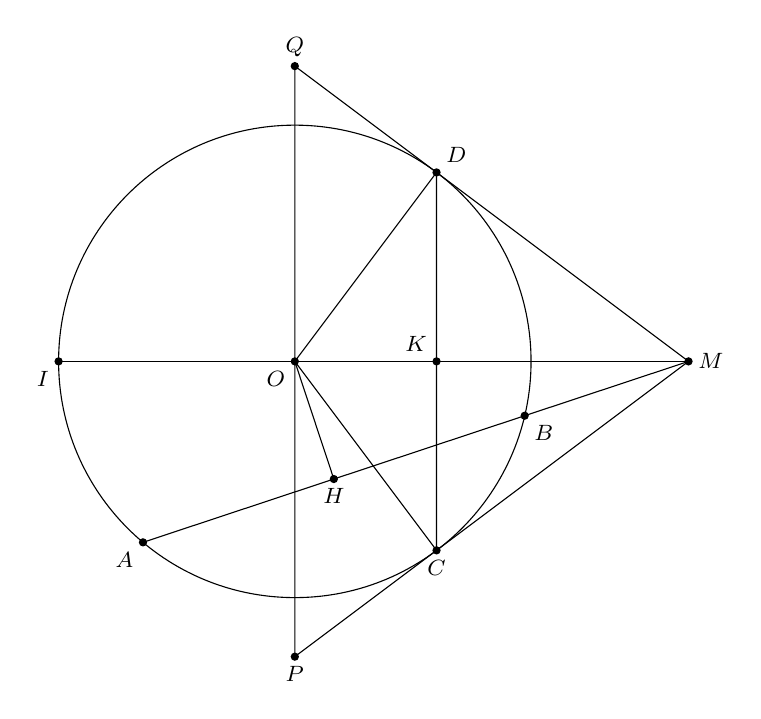
\begin{tikzpicture}[line join = round, line cap=round,>=stealth,font=\footnotesize,scale=1]
				\usetikzlibrary{calc}
				
				% Khai báo các giá trị cơ bản
				\def\r{3}
				\def\a{5}
				% acos trong pgfmath trả về giá trị bằng độ, phù hợp cho tọa độ cực của TikZ
				\pgfmathsetmacro{\alphaVal}{acos(\r/\a)}
				\pgfmathsetmacro{\kVal}{sqrt(\a*\a*\r*\r/(\a*\a-\r*\r))}
				
				% Định nghĩa tọa độ các điểm
				\coordinate (O) at (0,0);
				\coordinate (I) at (-\r,0);
				\coordinate (M) at (\a,0);
				\coordinate (D) at (\alphaVal:\r);      % D theo tọa độ cực (góc alphaVal, bán kính r)
				\coordinate (C) at (-\alphaVal:\r);     % C theo tọa độ cực (góc -alphaVal, bán kính r)
				\coordinate (Q) at (0, \kVal);        % Q(0,k)
				\coordinate (P) at (0, -\kVal);       % P(0,-k) - giả định từ Q(0,k) thứ hai
				\coordinate (A) at (-130:\r);         % A theo tọa độ cực
				
				% Các điểm được tính toán
				\coordinate (H) at ($(A)!(O)!(M)$);    % H là hình chiếu của O lên AM
				\coordinate (B) at ($2*(H)-(A)$);    % B sao cho H là trung điểm AB
				\coordinate (K) at ($(D)!0.5!(C)$);    % K là trung điểm DC
				
				% Vẽ các đối tượng hình học
				\draw (O) circle (\r);              % Đường tròn (O,r)
				\draw (P) -- (Q) -- (M) -- cycle;   % Tam giác PQM
				\draw (O) -- (D) -- (C) -- cycle;   % Tam giác ODC
				\draw (I) -- (M);                   % Đoạn thẳng IM
				\draw (M) -- (A);                   % Đoạn thẳng MA
				\draw (H) -- (O);                   % Đoạn thẳng HC
				
				% Tô màu và đặt nhãn cho các điểm
				\fill (O) circle (1.5pt);
				\fill (B) circle (1.5pt);
				\fill (I) circle (1.5pt);
				\fill (D) circle (1.5pt);
				\fill (C) circle (1.5pt);
				\fill (Q) circle (1.5pt);
				\fill (P) circle (1.5pt);
				\fill (A) circle (1.5pt);
				\fill (M) circle (1.5pt);
				\fill (H) circle (1.5pt);
				\fill (K) circle (1.5pt);
				
				\node[below left] at (O) {$O$};
				\node[below left] at (A) {$A$};
				\node[below right] at (B) {$B$};
				\node[below left] at (I) {$I$};
				\node[above right] at (D) {$D$};
				\node[below] at (C) {$C$};
				\node[above] at (Q) {$Q$};
				\node[below] at (P) {$P$};
				\node[right] at (M) {$M$};
				\node[below] at (H) {$H$};
				\node[above left] at (K) {$K$};
				
			\end{tikzpicture}
			
		\end{center}
		
		OM cắt CD tại K. Chứng minh $OK \cdot OM = R^2$. \\
		\\
		Ta có: Tam giác $ODM$ vuông tại $D$ (vì $\widehat{ODM} = 90^\circ$). \\
		Mặt khác: $MC = MD$ (Tính chất hai tiếp tuyến cắt nhau); \\
		$OC = OD = R$. \\
		Suy ra $OM$ là đường trung trực của đoạn thẳng $CD$ suy ra $OM \perp CD$. \\
		\\
		Trong tam giác vuông $ODM$ tại $D$ và tam giác $OKD$ đồng dạng (g-g) nên ta có: \\
		$OD^2 = OK \cdot OM$. \\
		suy ra $OK \cdot OM = R^2$. \\
		\\
		Theo t/c hai tiếp tuyến cắt nhau ta có $MO$ là tia phân giác của góc $PMQ$, mặt \\
		khác $MO \perp PQ$ nên tam giác $PMQ$ cân tại $M$ suy ra $PQ = 2OP$. \\
		\\
		Ta có $S_{PMQ} = \frac{1}{2} MO \cdot PQ = MO \cdot OP$. \\
		\\
		Trong tam giác vuông $OMP$ ta có: $OC \cdot PM = OP \cdot OM$. \\
		$\Rightarrow OC^2 \cdot PM^2 = OP^2 \cdot OM^2$ \\
		\\
		$\frac{1}{OC^2} = \frac{1}{OP^2} + \frac{1}{OM^2}$ suy ra $\frac{1}{R^2} = \frac{1}{OP^2} + \frac{1}{OM^2}$. \\
		\\
		Áp dụng bất đẳng thức Cô si : \\
		$\frac{1}{OP^2} + \frac{1}{OM^2} \ge 2 \sqrt{\frac{1}{OP^2} \cdot \frac{1}{OM^2}} = \frac{2}{OP \cdot OM}$ suy ra $\frac{1}{R^2} \ge \frac{2}{S_{PMQ}}$. \\
		\\
		$S_{PMQ} \ge 2R^2$. Dấu “=” xảy ra khi
		$\begin{cases}
			\frac{1}{OP^2} = \frac{1}{OM^2} \\
			OM \cdot OP = 2R^2
		\end{cases}$
		suy ra $OM = OP = R\sqrt{2}$. \\
		\\
		Vậy $S_{PMQ}$ đạt giá trị nhỏ nhất khi $OM = R\sqrt{2}$.
	}
	
	
\end{ex}

\begin{ex} % Câu 14
	\begin{enumerate}
		\item[a)] Bạn Thắng có $n$ tấm thẻ cùng loại được đánh số từ $1$ đến $n$. Bạn Thắng rút ngẫu nhiên 1 tấm thẻ. Biết rằng xác suất của biến cố “Lấy được tấm thẻ ghi số có một chữ số là $0,18$. Hỏi bạn Thắng có bao nhiêu tấm thẻ?
		\item[b)] Cho ba số dương $a, b, c$ thỏa mãn $ab + bc + ca = 1$. Chứng minh rằng:
		$$ \frac{\sqrt{a^2+1}-a}{bc} + \frac{\sqrt{b^2+1}-b}{ac} + \frac{\sqrt{c^2+1}-c}{ab} \le \frac{1}{a} + \frac{1}{b} + \frac{1}{c} $$
	\end{enumerate}
	
	
\end{ex}
	


\setcounterref{ex}{0}